\documentclass{article}

\usepackage[a4paper, bottom=0.5in, top=0.5in, left=0.5in, right=0.5in]{geometry}
\usepackage{wrapfig}
\usepackage{natbib}
\usepackage{url}
\usepackage{xcolor}
\usepackage{caption}
\usepackage{hyperref}
\hypersetup{
    colorlinks=true,    
    urlcolor=cyan,
}
\usepackage{bytefield}

\usepackage{amsfonts}
\usepackage{float}
\usepackage{enumitem}

\usepackage{tikz-timing}[2014/10/29]
\usetikztiminglibrary[rising arrows]{clockarrows}

\usepackage{minted}

\usepackage{xparse} % NewDocumentCommand, IfValueTF, IFBooleanTF
\usepackage{tikz-timing}[2014/10/29]
\NewDocumentCommand{\busref}{som}{\texttt{%
		#3%
		\IfValueTF{#2}{[#2]}{}%
		\IfBooleanTF{#1}{\#}{}%
}}


\newcommand{\bitFormat}[1]{\emph{\textbf{\textcolor{cyan}{#1}}}}

\newcommand{\regFormat}[1]{\textbf{\textcolor{magenta}{#1}}}

\newcommand{\pinFormat}[1]{\emph{\textcolor{red}{#1}}}


\usepackage{graphicx}
\graphicspath{ {./Resources/pics/} }



\title{ATmega328P USART0}
\author{Narendiran S}
\date{\today}

\begin{document}
\maketitle

\section{Features}
\begin{itemize}
    \item Full duplex operation (independent serial receive and transmit registers).
    \item Asynchronous or synchronous operation
    \item High resolution baud rate generator
    \item Serial frame with 5,6,7,8,9 data bits and 1 or 2 stop bits
    \item Odd or even partiy generator and checker by hardware
    \item Double speed asynchronous communication mode
\end{itemize}
\section{Block Diagram}
\begin{figure}[H]
    \centering
    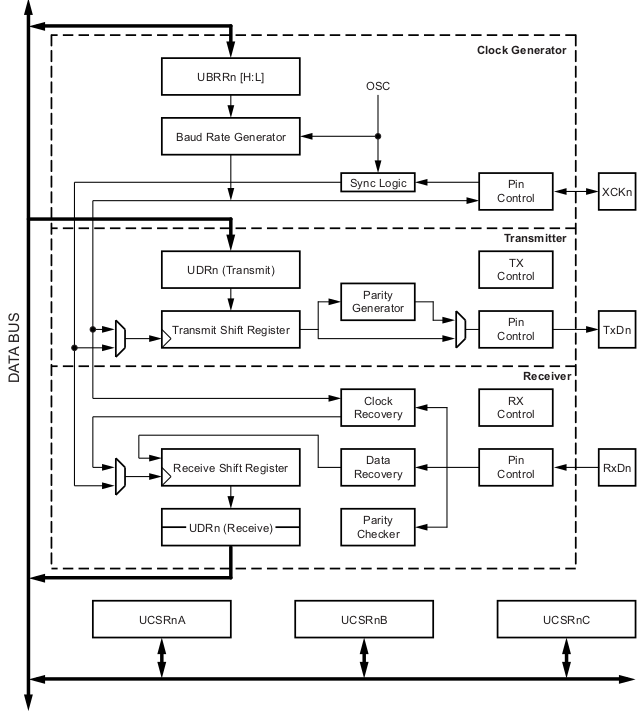
\includegraphics[height=0.58\textheight]{USART0BlockDiagram.png}
\end{figure}

\subsection{Clock Generator Block}
\begin{itemize}
    \item Consist of sync. Logic for external clock input for usage in sync. slave operation 
    \item Consist of Baud rate Generator.
    \item Uses the \pinFormat{XCKn} pin for sync. Transfer mode
\end{itemize}

\subsection{Transmitte Block}
\begin{itemize}
    \item Consist of singe write buffer – continuous transfer of data without delay between frames
    \item Consist of Serial Shift register and Parity Generator
    \item Also, Control logic for handling different serial frame format.
\end{itemize}

\subsection{Receiver Block}
\begin{itemize}
    \item Consist of Clock and data recovery unit – uses for Asynchronous reception
    \item Consist of Parity Checker, Control Logic, Shift Register, Two level Receiver buffer
    \item Can support frame error, data overrun parity error
\end{itemize}

\section{Clock Genration}
\begin{figure}[H]
    \centering
    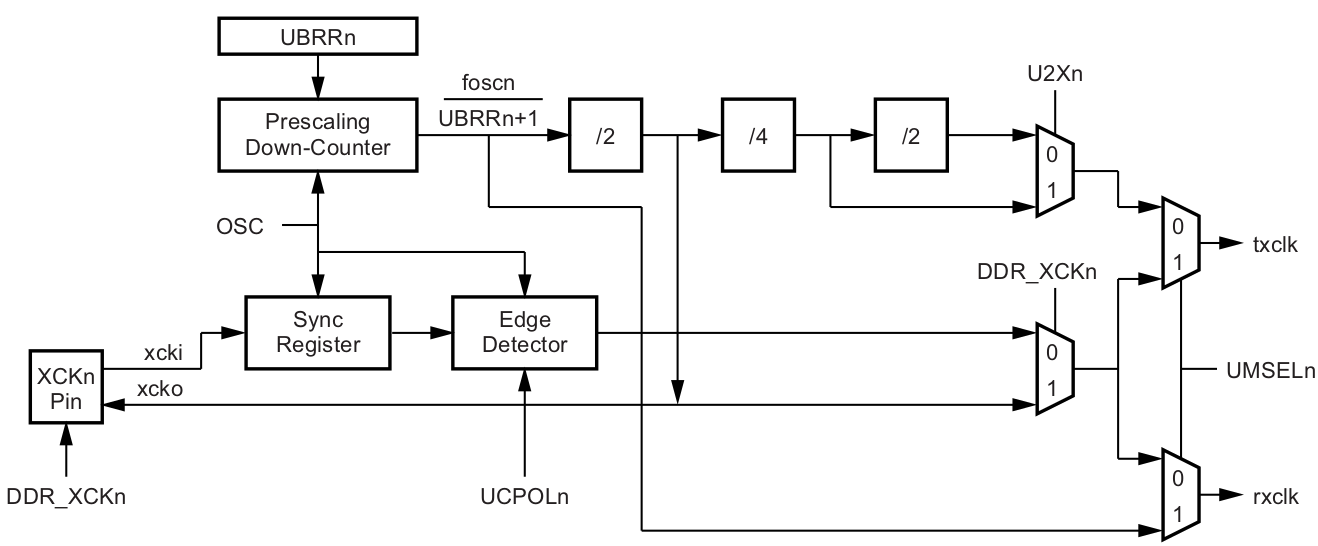
\includegraphics[width=1\textwidth]{USART0ClockGeneration.png}
\end{figure}
\begin{itemize}
    \item Generates Base Clock for Transmitter and Receiver.
    \item USART supports four modes of clock operation
    \begin{enumerate}[label=(\roman*)]
        \item Normal Asynchronous
        \item Double Speed Asynchronous
        \item Master synchronous
        \item Slave synchronous
    \end{enumerate}
    \item Selection between Asynchronous and Synchronous is done by \bitFormat{UMSELn} bit in \bitFormat{UCSRnC} - USART Control and Status Register C.
    \item The Double Speed is selected by \bitFormat{U2Xn} bit in \bitFormat{UCSRnA} - USART Control and Status Register A.
    \item In Synchronous Mode, the master or slave mode is selected by \bitFormat{DDR\_XSCn} bit direction. [external - slave mode; internal - master mode]
\end{itemize}
\begin{table}[H]
    \begin{center}
        \begin{tabular}{c|c}
            \textbf{Signals} & \textbf{Description}\\
            \hline
            txclk & Transmitte Clock\\
            rxclk & Receiver Base Clock\\
            xclki & Input from \pinFormat{XCK} pin - used for synchronous slave operation.\\
            xclko & Clock output to \pinFormat{XCK} pin - used for synchronous master operation.\\
            fosc & \pinFormat{XTAL} pin freqency (System clock).
        \end{tabular}
    \end{center}
\end{table}

\subsection{Internal Clock Generation - The Baud Rate Generator}
\begin{itemize}
    \item Used for Asynchronous and Synchronous Master modes of operation.
    \item Programmed using \regFormat{UBRRn} register.
\end{itemize}

\begin{table}[H]
    \begin{center}
        \begin{tabular}{c|c}
            \textbf{Operating Mode} & \textbf{UBRRn calculation}\\
            \hline
            Asynchronous Normal Mode(\bitFormat{U2Xn} == 0) & $UBRRn = \frac{f_{OSC}}{16 * BAUD} - 1$\\
            Asynchronous Double Speed Mode(\bitFormat{U2Xn} == 1) & $UBRRn = \frac{f_{OSC}}{8 * BAUD} - 1$\\
            Synchronous Master Mode & $UBRRn = \frac{f_{OSC}}{2 * BAUD} - 1$\\
        \end{tabular}
    \end{center}
\end{table}

\subsection{External Clock}
\begin{itemize}
    \item Used by synchronous Slave mode.
    \item External clock input from \pinFormat{XCKn} pin is used and should
\end{itemize}
\begin{center}
    $f_{XCK} < \frac{f_{OSC}}{4}$
\end{center}

\section{Frame Format}
\begin{figure}[H]
    \centering
    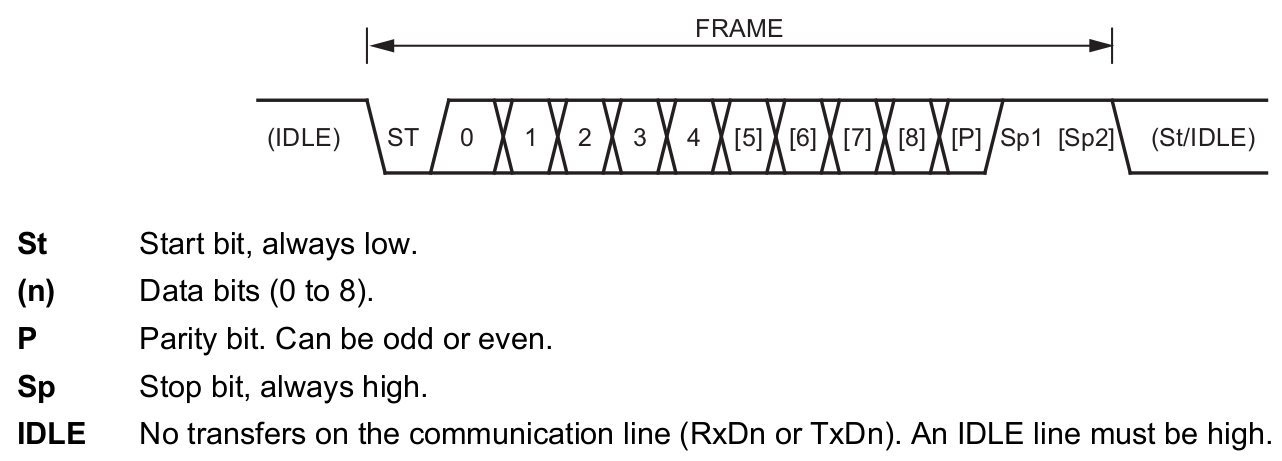
\includegraphics[width=1\textwidth]{USART0FrameFormat.png}
\end{figure}
\begin{itemize}
    \item A serial frame is defined to be one character of data bits with synchronization bits (start and stop bits), and optionally a parity bit for error checking.
    \item The combinations can be
    \begin{itemize}
        \item 1 start bit
        \item 5 or 6 or 7 or 8 or 9 data bits
        \item no or even or odd parity bits
        \item 1 or 2 stop bits
    \end{itemize}
    \item A frame starts with start bit followed by LSB data bits.
    \item Next the data bet can be from 5 to 9 ending with MSB data bits.
    \item Parity bits may be added if enabled.
    \item Finally, stop bit of 1 or 2 size is added.
    \item Generally, the line is idel with high Logic.
\end{itemize}
\section{Register Description}
\subsection*{UDRn – USART I/O Data Register n}
\vspace*{0.5cm}
\begin{bytefield}[bitformatting={\large\bfseries},
    endianness=big,bitwidth=0.125\linewidth]{8}
    \bitheader[lsb=0]{0-7} \\
    \bitbox{8}{\small RXB[7:0]}\\
    \bitbox{8}{\small TXB[7:0]}\\
\end{bytefield}

\subsubsection*{UCSRnA – USART Control and Status Register n A}
\vspace*{0.5cm}
\begin{bytefield}[bitformatting={\large\bfseries},
    endianness=big,bitwidth=0.125\linewidth]{8}
    \bitheader[lsb=0]{0-7} \\
    \bitbox{1}{\small RXCn}
    \bitbox{1}{\small TXCn}
    \bitbox{1}{\small UDREn}
    \bitbox{1}{\small FEn}
    \bitbox{1}{\small DORn}
    \bitbox{1}{\small UPEn}
    \bitbox{1}{\small U2Xn}
    \bitbox{1}{\small MPCMn}\\
\end{bytefield}
\begin{itemize}
    \item \bitFormat{RXCn} - USART Receive Complete - Set when there are unread data in receive buffer.
    \item \bitFormat{TXCn} - USART Transmit Complete - Set when the entire frame in the transmit shift register has been shifted out and there are no new data currently present in the transmit buffer.
    \item \bitFormat{UDREn} - USART Data Register Empty - indicates if the transmit buffer is ready to receive new data. A one indicates buffer is expty and ready to transmit.
    \item \bitFormat{U2Xn:} - Double the USART Transmission Speed - Affects only the asynchronous operation. One will increase the speeed of transfer rate in asynchronous opration.
\end{itemize}

\end{document}